\documentclass[1p]{elsarticle_modified}
%\bibliographystyle{elsarticle-num}

%\usepackage[colorlinks]{hyperref}
%\usepackage{abbrmath_seonhwa} %\Abb, \Ascr, \Acal ,\Abf, \Afrak
\usepackage{amsfonts}
\usepackage{amssymb}
\usepackage{amsmath}
\usepackage{amsthm}
\usepackage{scalefnt}
\usepackage{amsbsy}
\usepackage{kotex}
\usepackage{caption}
\usepackage{subfig}
\usepackage{color}
\usepackage{graphicx}
\usepackage{xcolor} %% white, black, red, green, blue, cyan, magenta, yellow
\usepackage{float}
\usepackage{setspace}
\usepackage{hyperref}

\usepackage{tikz}
\usetikzlibrary{arrows}

\usepackage{multirow}
\usepackage{array} % fixed length table
\usepackage{hhline}

%%%%%%%%%%%%%%%%%%%%%
\makeatletter
\renewcommand*\env@matrix[1][\arraystretch]{%
	\edef\arraystretch{#1}%
	\hskip -\arraycolsep
	\let\@ifnextchar\new@ifnextchar
	\array{*\c@MaxMatrixCols c}}
\makeatother %https://tex.stackexchange.com/questions/14071/how-can-i-increase-the-line-spacing-in-a-matrix
%%%%%%%%%%%%%%%

\usepackage[normalem]{ulem}

\newcommand{\msout}[1]{\ifmmode\text{\sout{\ensuremath{#1}}}\else\sout{#1}\fi}
%SOURCE: \msout is \stkout macro in https://tex.stackexchange.com/questions/20609/strikeout-in-math-mode

\newcommand{\cancel}[1]{
	\ifmmode
	{\color{red}\msout{#1}}
	\else
	{\color{red}\sout{#1}}
	\fi
}

\newcommand{\add}[1]{
	{\color{blue}\uwave{#1}}
}

\newcommand{\replace}[2]{
	\ifmmode
	{\color{red}\msout{#1}}{\color{blue}\uwave{#2}}
	\else
	{\color{red}\sout{#1}}{\color{blue}\uwave{#2}}
	\fi
}

\newcommand{\Sol}{\mathcal{S}} %segment
\newcommand{\D}{D} %diagram
\newcommand{\A}{\mathcal{A}} %arc


%%%%%%%%%%%%%%%%%%%%%%%%%%%%%5 test

\def\sl{\operatorname{\textup{SL}}(2,\Cbb)}
\def\psl{\operatorname{\textup{PSL}}(2,\Cbb)}
\def\quan{\mkern 1mu \triangleright \mkern 1mu}

\theoremstyle{definition}
\newtheorem{thm}{Theorem}[section]
\newtheorem{prop}[thm]{Proposition}
\newtheorem{lem}[thm]{Lemma}
\newtheorem{ques}[thm]{Question}
\newtheorem{cor}[thm]{Corollary}
\newtheorem{defn}[thm]{Definition}
\newtheorem{exam}[thm]{Example}
\newtheorem{rmk}[thm]{Remark}
\newtheorem{alg}[thm]{Algorithm}

\newcommand{\I}{\sqrt{-1}}
\begin{document}

%\begin{frontmatter}
%
%\title{Boundary parabolic representations of knots up to 8 crossings}
%
%%% Group authors per affiliation:
%\author{Yunhi Cho} 
%\address{Department of Mathematics, University of Seoul, Seoul, Korea}
%\ead{yhcho@uos.ac.kr}
%
%
%\author{Seonhwa Kim} %\fnref{s_kim}}
%\address{Center for Geometry and Physics, Institute for Basic Science, Pohang, 37673, Korea}
%\ead{ryeona17@ibs.re.kr}
%
%\author{Hyuk Kim}
%\address{Department of Mathematical Sciences, Seoul National University, Seoul 08826, Korea}
%\ead{hyukkim@snu.ac.kr}
%
%\author{Seokbeom Yoon}
%\address{Department of Mathematical Sciences, Seoul National University, Seoul, 08826,  Korea}
%\ead{sbyoon15@snu.ac.kr}
%
%\begin{abstract}
%We find all boundary parabolic representation of knots up to 8 crossings.
%
%\end{abstract}
%\begin{keyword}
%    \MSC[2010] 57M25 
%\end{keyword}
%
%\end{frontmatter}

%\linenumbers
%\tableofcontents
%
\newcommand\colored[1]{\textcolor{white}{\rule[-0.35ex]{0.8em}{1.4ex}}\kern-0.8em\color{red} #1}%
%\newcommand\colored[1]{\textcolor{white}{ #1}\kern-2.17ex	\textcolor{white}{ #1}\kern-1.81ex	\textcolor{white}{ #1}\kern-2.15ex\color{red}#1	}

{\Large $\underline{12a_{1261}~(K12a_{1261})}$}

\setlength{\tabcolsep}{10pt}
\renewcommand{\arraystretch}{1.6}
\vspace{1cm}\begin{tabular}{m{100pt}>{\centering\arraybackslash}m{274pt}}
\multirow{5}{120pt}{
	\centering
	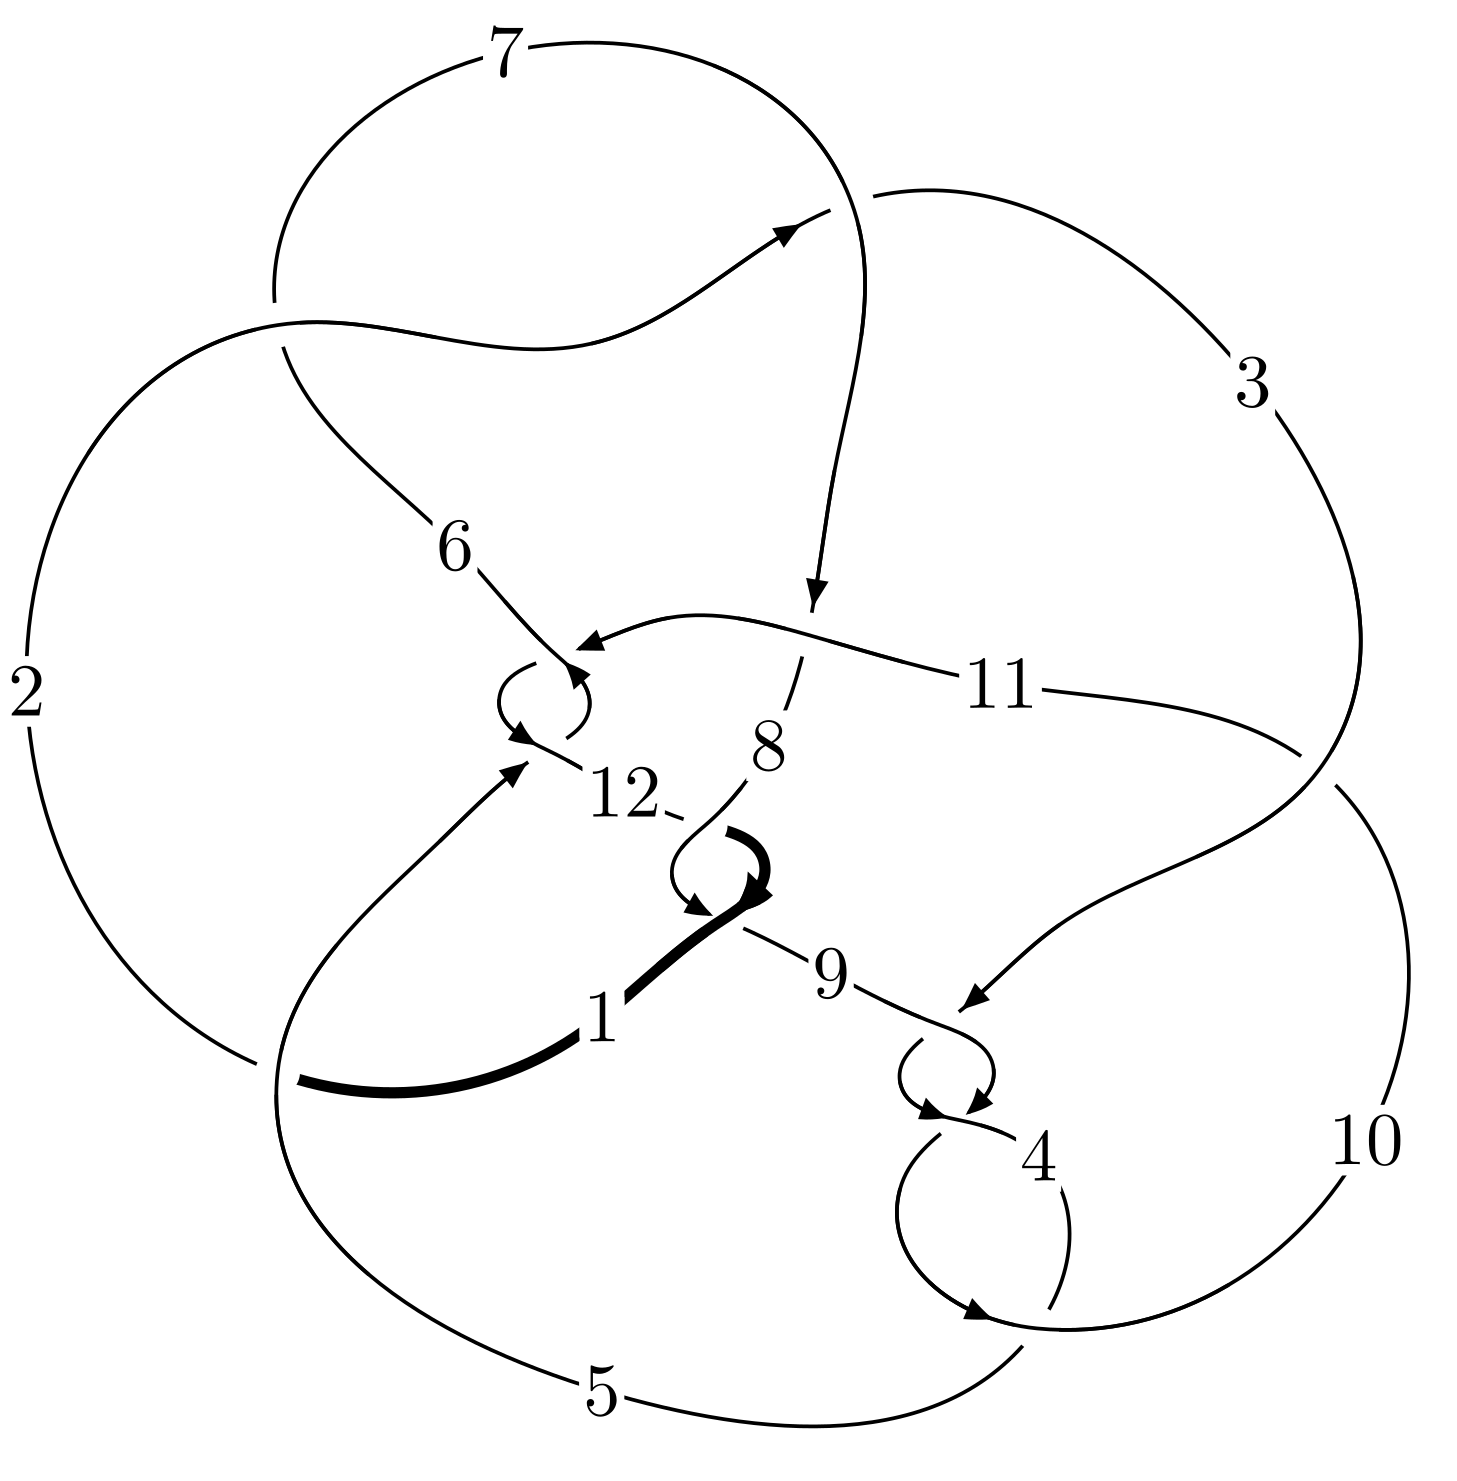
\includegraphics[width=112pt]{../../../GIT/diagram.site/Diagrams/png/2062_12a_1261.png}\\
\ \ \ A knot diagram\footnotemark}&
\allowdisplaybreaks
\textbf{Linearized knot diagam} \\
\cline{2-2}
 &
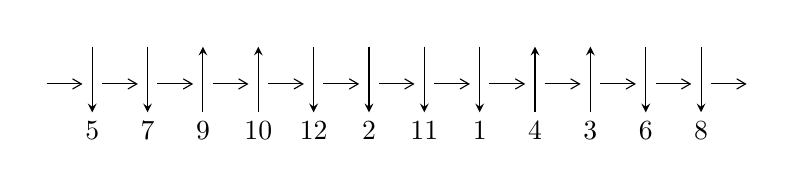
\begin{tikzpicture}[x=20pt, y=17pt]
	% nodes
	\node (C0) at (0, 0) {};
	\node (C1) at (1, 0) {};
	\node (C1U) at (1, +1) {};
	\node (C1D) at (1, -1) {5};

	\node (C2) at (2, 0) {};
	\node (C2U) at (2, +1) {};
	\node (C2D) at (2, -1) {7};

	\node (C3) at (3, 0) {};
	\node (C3U) at (3, +1) {};
	\node (C3D) at (3, -1) {9};

	\node (C4) at (4, 0) {};
	\node (C4U) at (4, +1) {};
	\node (C4D) at (4, -1) {10};

	\node (C5) at (5, 0) {};
	\node (C5U) at (5, +1) {};
	\node (C5D) at (5, -1) {12};

	\node (C6) at (6, 0) {};
	\node (C6U) at (6, +1) {};
	\node (C6D) at (6, -1) {2};

	\node (C7) at (7, 0) {};
	\node (C7U) at (7, +1) {};
	\node (C7D) at (7, -1) {11};

	\node (C8) at (8, 0) {};
	\node (C8U) at (8, +1) {};
	\node (C8D) at (8, -1) {1};

	\node (C9) at (9, 0) {};
	\node (C9U) at (9, +1) {};
	\node (C9D) at (9, -1) {4};

	\node (C10) at (10, 0) {};
	\node (C10U) at (10, +1) {};
	\node (C10D) at (10, -1) {3};

	\node (C11) at (11, 0) {};
	\node (C11U) at (11, +1) {};
	\node (C11D) at (11, -1) {6};

	\node (C12) at (12, 0) {};
	\node (C12U) at (12, +1) {};
	\node (C12D) at (12, -1) {8};
	\node (C13) at (13, 0) {};

	% arrows
	\draw[->,>={angle 60}]
	(C0) edge (C1) (C1) edge (C2) (C2) edge (C3) (C3) edge (C4) (C4) edge (C5) (C5) edge (C6) (C6) edge (C7) (C7) edge (C8) (C8) edge (C9) (C9) edge (C10) (C10) edge (C11) (C11) edge (C12) (C12) edge (C13) ;	\draw[->,>=stealth]
	(C1U) edge (C1D) (C2U) edge (C2D) (C3D) edge (C3U) (C4D) edge (C4U) (C5U) edge (C5D) (C6U) edge (C6D) (C7U) edge (C7D) (C8U) edge (C8D) (C9D) edge (C9U) (C10D) edge (C10U) (C11U) edge (C11D) (C12U) edge (C12D) ;
	\end{tikzpicture} \\
\hhline{~~} \\& 
\textbf{Solving Sequence} \\ \cline{2-2} 
 &
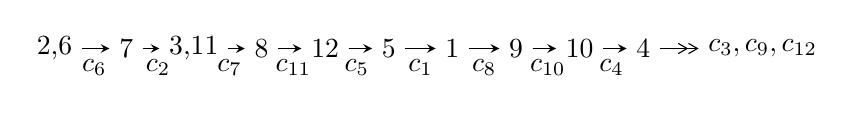
\begin{tikzpicture}[x=23pt, y=7pt]
	% node
	\node (A0) at (-1/8, 0) {2,6};
	\node (A1) at (1, 0) {7};
	\node (A2) at (33/16, 0) {3,11};
	\node (A3) at (25/8, 0) {8};
	\node (A4) at (33/8, 0) {12};
	\node (A5) at (41/8, 0) {5};
	\node (A6) at (49/8, 0) {1};
	\node (A7) at (57/8, 0) {9};
	\node (A8) at (65/8, 0) {10};
	\node (A9) at (73/8, 0) {4};
	\node (C1) at (1/2, -1) {$c_{6}$};
	\node (C2) at (3/2, -1) {$c_{2}$};
	\node (C3) at (21/8, -1) {$c_{7}$};
	\node (C4) at (29/8, -1) {$c_{11}$};
	\node (C5) at (37/8, -1) {$c_{5}$};
	\node (C6) at (45/8, -1) {$c_{1}$};
	\node (C7) at (53/8, -1) {$c_{8}$};
	\node (C8) at (61/8, -1) {$c_{10}$};
	\node (C9) at (69/8, -1) {$c_{4}$};
	\node (A10) at (11, 0) {$c_{3},c_{9},c_{12}$};

	% edge
	\draw[->,>=stealth]	
	(A0) edge (A1) (A1) edge (A2) (A2) edge (A3) (A3) edge (A4) (A4) edge (A5) (A5) edge (A6) (A6) edge (A7) (A7) edge (A8) (A8) edge (A9) ;
	\draw[->>,>={angle 60}]	
	(A9) edge (A10);
\end{tikzpicture} \\ 

\end{tabular} \\

\footnotetext{
The image of knot diagram is generated by the software ``\textbf{Draw programme}" developed by Andrew Bartholomew(\url{http://www.layer8.co.uk/maths/draw/index.htm\#Running-draw}), where we modified some parts for our purpose(\url{https://github.com/CATsTAILs/LinksPainter}).
}\phantom \\ \newline 
\centering \textbf{Ideals for irreducible components\footnotemark of $X_{\text{par}}$} 
 
\begin{align*}
I^u_{1}&=\langle 
-6.86400\times10^{38} u^{39}+1.22276\times10^{38} u^{38}+\cdots+1.38766\times10^{39} b+6.71756\times10^{39},\\
\phantom{I^u_{1}}&\phantom{= \langle  }-1.41733\times10^{40} u^{39}+5.75302\times10^{39} u^{38}+\cdots+1.38766\times10^{40} a+1.26988\times10^{41},\;u^{40}- u^{39}+\cdots-8 u+5\rangle \\
I^u_{2}&=\langle 
1.49972\times10^{95} u^{63}-1.89102\times10^{95} u^{62}+\cdots+1.42532\times10^{96} b-6.59620\times10^{93},\\
\phantom{I^u_{2}}&\phantom{= \langle  }-9.36179\times10^{96} u^{63}+6.79343\times10^{96} u^{62}+\cdots+7.12662\times10^{96} a-8.34927\times10^{96},\;u^{64}- u^{63}+\cdots+2 u-1\rangle \\
I^u_{3}&=\langle 
b+u,\;8 a^3-12 a^2 u+4 a^2-4 a u-6 a+u-2,\;u^2+1\rangle \\
I^u_{4}&=\langle 
b,\;a+1,\;u+1\rangle \\
\\
\end{align*}
\raggedright * 4 irreducible components of $\dim_{\mathbb{C}}=0$, with total 111 representations.\\
\footnotetext{All coefficients of polynomials are rational numbers. But the coefficients are sometimes approximated in decimal forms when there is not enough margin.}
\newpage
\renewcommand{\arraystretch}{1}
\centering \section*{I. $I^u_{1}= \langle -6.86\times10^{38} u^{39}+1.22\times10^{38} u^{38}+\cdots+1.39\times10^{39} b+6.72\times10^{39},\;-1.42\times10^{40} u^{39}+5.75\times10^{39} u^{38}+\cdots+1.39\times10^{40} a+1.27\times10^{41},\;u^{40}- u^{39}+\cdots-8 u+5 \rangle$}
\flushleft \textbf{(i) Arc colorings}\\
\begin{tabular}{m{7pt} m{180pt} m{7pt} m{180pt} }
\flushright $a_{2}=$&$\begin{pmatrix}0\\u\end{pmatrix}$ \\
\flushright $a_{6}=$&$\begin{pmatrix}1\\0\end{pmatrix}$ \\
\flushright $a_{7}=$&$\begin{pmatrix}1\\u^2\end{pmatrix}$ \\
\flushright $a_{3}=$&$\begin{pmatrix}- u\\- u^3+u\end{pmatrix}$ \\
\flushright $a_{11}=$&$\begin{pmatrix}1.02138 u^{39}-0.414584 u^{38}+\cdots+4.29657 u-9.15125\\0.494646 u^{39}-0.0881164 u^{38}+\cdots+2.78143 u-4.84092\end{pmatrix}$ \\
\flushright $a_{8}=$&$\begin{pmatrix}0.232933 u^{39}-0.199072 u^{38}+\cdots-0.626073 u-2.92962\\0.200267 u^{39}-0.138012 u^{38}+\cdots-0.0964501 u-2.63367\end{pmatrix}$ \\
\flushright $a_{12}=$&$\begin{pmatrix}0.526734 u^{39}-0.326467 u^{38}+\cdots+1.51515 u-4.31032\\0.494646 u^{39}-0.0881164 u^{38}+\cdots+2.78143 u-4.84092\end{pmatrix}$ \\
\flushright $a_{5}=$&$\begin{pmatrix}0.361388 u^{39}-0.0370447 u^{38}+\cdots+1.83025 u+0.142855\\0.407986 u^{39}-0.0703407 u^{38}+\cdots+1.54549 u-0.676271\end{pmatrix}$ \\
\flushright $a_{1}=$&$\begin{pmatrix}0.492873 u^{39}-0.140306 u^{38}+\cdots+2.58130 u-3.14566\\0.432390 u^{39}+0.0156258 u^{38}+\cdots+3.81296 u-3.83959\end{pmatrix}$ \\
\flushright $a_{9}=$&$\begin{pmatrix}0.585500 u^{39}-0.322926 u^{38}+\cdots+0.171255 u-5.39399\\0.648283 u^{39}-0.410746 u^{38}+\cdots-0.476912 u-4.79562\end{pmatrix}$ \\
\flushright $a_{10}=$&$\begin{pmatrix}0.633625 u^{39}-0.286109 u^{38}+\cdots+3.62724 u-4.52753\\0.902893 u^{39}-0.249069 u^{38}+\cdots+3.31529 u-8.16823\end{pmatrix}$ \\
\flushright $a_{4}=$&$\begin{pmatrix}0.148813 u^{39}-0.00235840 u^{38}+\cdots+0.508516 u+0.427860\\-0.524790 u^{39}+0.102722 u^{38}+\cdots-1.39513 u+3.44351\end{pmatrix}$\\&\end{tabular}
\flushleft \textbf{(ii) Obstruction class $= -1$}\\~\\
\flushleft \textbf{(iii) Cusp Shapes $= 0.246686 u^{39}+0.293708 u^{38}+\cdots+1.39766 u-6.81633$}\\~\\
\newpage\renewcommand{\arraystretch}{1}
\flushleft \textbf{(iv) u-Polynomials at the component}\newline \\
\begin{tabular}{m{50pt}|m{274pt}}
Crossings & \hspace{64pt}u-Polynomials at each crossing \\
\hline $$\begin{aligned}c_{1},c_{7}\end{aligned}$$&$\begin{aligned}
&64(64 u^{40}+128 u^{39}+\cdots-18 u+4)
\end{aligned}$\\
\hline $$\begin{aligned}c_{2},c_{6},c_{8}\\c_{12}\end{aligned}$$&$\begin{aligned}
&u^{40}- u^{39}+\cdots-8 u+5
\end{aligned}$\\
\hline $$\begin{aligned}c_{3},c_{4},c_{9}\end{aligned}$$&$\begin{aligned}
&u^{40}-3 u^{39}+\cdots+40 u+10
\end{aligned}$\\
\hline $$\begin{aligned}c_{5},c_{11}\end{aligned}$$&$\begin{aligned}
&u^{40}-3 u^{39}+\cdots-116 u+178
\end{aligned}$\\
\hline $$\begin{aligned}c_{10}\end{aligned}$$&$\begin{aligned}
&u^{40}+9 u^{39}+\cdots+223540 u+24310
\end{aligned}$\\
\hline
\end{tabular}\\~\\
\newpage\renewcommand{\arraystretch}{1}
\flushleft \textbf{(v) Riley Polynomials at the component}\newline \\
\begin{tabular}{m{50pt}|m{274pt}}
Crossings & \hspace{64pt}Riley Polynomials at each crossing \\
\hline $$\begin{aligned}c_{1},c_{7}\end{aligned}$$&$\begin{aligned}
&4096(4096 y^{40}-16384 y^{39}+\cdots+4 y+16)
\end{aligned}$\\
\hline $$\begin{aligned}c_{2},c_{6},c_{8}\\c_{12}\end{aligned}$$&$\begin{aligned}
&y^{40}-15 y^{39}+\cdots-64 y+25
\end{aligned}$\\
\hline $$\begin{aligned}c_{3},c_{4},c_{9}\end{aligned}$$&$\begin{aligned}
&y^{40}-33 y^{39}+\cdots-140 y+100
\end{aligned}$\\
\hline $$\begin{aligned}c_{5},c_{11}\end{aligned}$$&$\begin{aligned}
&y^{40}+23 y^{39}+\cdots+897548 y+31684
\end{aligned}$\\
\hline $$\begin{aligned}c_{10}\end{aligned}$$&$\begin{aligned}
&y^{40}+19 y^{39}+\cdots-3244220940 y+590976100
\end{aligned}$\\
\hline
\end{tabular}\\~\\
\newpage\flushleft \textbf{(vi) Complex Volumes and Cusp Shapes}
$$\begin{array}{c|c|c}  
\text{Solutions to }I^u_{1}& \I (\text{vol} + \sqrt{-1}CS) & \text{Cusp shape}\\
 \hline 
\begin{aligned}
u &= \phantom{-}0.951302 + 0.290221 I \\
a &= -0.277187 - 0.863557 I \\
b &= \phantom{-}0.11645 - 1.69893 I\end{aligned}
 & \phantom{-}2.44631 - 5.94320 I & -2.32452 + 10.00245 I \\ \hline\begin{aligned}
u &= \phantom{-}0.951302 - 0.290221 I \\
a &= -0.277187 + 0.863557 I \\
b &= \phantom{-}0.11645 + 1.69893 I\end{aligned}
 & \phantom{-}2.44631 + 5.94320 I & -2.32452 - 10.00245 I \\ \hline\begin{aligned}
u &= -0.986545 + 0.209518 I \\
a &= -1.94798 + 0.60057 I \\
b &= -1.21607 + 1.07214 I\end{aligned}
 & -2.78388 + 2.32701 I & -5.94560 - 9.38612 I \\ \hline\begin{aligned}
u &= -0.986545 - 0.209518 I \\
a &= -1.94798 - 0.60057 I \\
b &= -1.21607 - 1.07214 I\end{aligned}
 & -2.78388 - 2.32701 I & -5.94560 + 9.38612 I \\ \hline\begin{aligned}
u &= \phantom{-}0.359550 + 0.837445 I \\
a &= -0.225374 + 0.398951 I \\
b &= \phantom{-}0.114727 - 1.121370 I\end{aligned}
 & \phantom{-}3.64892 - 0.52199 I & \phantom{-}4.59024 + 2.59542 I \\ \hline\begin{aligned}
u &= \phantom{-}0.359550 - 0.837445 I \\
a &= -0.225374 - 0.398951 I \\
b &= \phantom{-}0.114727 + 1.121370 I\end{aligned}
 & \phantom{-}3.64892 + 0.52199 I & \phantom{-}4.59024 - 2.59542 I \\ \hline\begin{aligned}
u &= -0.839767 + 0.098563 I \\
a &= \phantom{-}0.96828 - 1.28580 I \\
b &= \phantom{-}0.39640 - 1.74102 I\end{aligned}
 & -1.26065 + 0.86355 I & \phantom{-}1.74294 - 5.70273 I \\ \hline\begin{aligned}
u &= -0.839767 - 0.098563 I \\
a &= \phantom{-}0.96828 + 1.28580 I \\
b &= \phantom{-}0.39640 + 1.74102 I\end{aligned}
 & -1.26065 - 0.86355 I & \phantom{-}1.74294 + 5.70273 I \\ \hline\begin{aligned}
u &= \phantom{-}1.111420 + 0.352542 I \\
a &= \phantom{-}1.72549 + 0.41631 I \\
b &= \phantom{-}0.89022 + 1.22122 I\end{aligned}
 & -2.02045 - 7.48389 I & -6.59522 + 9.84827 I \\ \hline\begin{aligned}
u &= \phantom{-}1.111420 - 0.352542 I \\
a &= \phantom{-}1.72549 - 0.41631 I \\
b &= \phantom{-}0.89022 - 1.22122 I\end{aligned}
 & -2.02045 + 7.48389 I & -6.59522 - 9.84827 I\\
 \hline 
 \end{array}$$\newpage$$\begin{array}{c|c|c}  
\text{Solutions to }I^u_{1}& \I (\text{vol} + \sqrt{-1}CS) & \text{Cusp shape}\\
 \hline 
\begin{aligned}
u &= -0.690269 + 0.961401 I \\
a &= \phantom{-}0.092925 + 0.142714 I \\
b &= -0.264351 - 1.186530 I\end{aligned}
 & \phantom{-}8.68492 + 1.39150 I & \phantom{-}3.97132 - 0.73814 I \\ \hline\begin{aligned}
u &= -0.690269 - 0.961401 I \\
a &= \phantom{-}0.092925 - 0.142714 I \\
b &= -0.264351 + 1.186530 I\end{aligned}
 & \phantom{-}8.68492 - 1.39150 I & \phantom{-}3.97132 + 0.73814 I \\ \hline\begin{aligned}
u &= -1.093880 + 0.546781 I \\
a &= -1.82594 + 0.17728 I \\
b &= -0.711478 + 1.169160 I\end{aligned}
 & \phantom{-}5.41370 + 9.49132 I & -1.05941 - 8.20262 I \\ \hline\begin{aligned}
u &= -1.093880 - 0.546781 I \\
a &= -1.82594 - 0.17728 I \\
b &= -0.711478 - 1.169160 I\end{aligned}
 & \phantom{-}5.41370 - 9.49132 I & -1.05941 + 8.20262 I \\ \hline\begin{aligned}
u &= -1.217690 + 0.271137 I \\
a &= \phantom{-}1.46583 + 0.49454 I \\
b &= \phantom{-}1.358560 + 0.314654 I\end{aligned}
 & -6.64670 + 2.06191 I & -9.67039 - 3.16010 I \\ \hline\begin{aligned}
u &= -1.217690 - 0.271137 I \\
a &= \phantom{-}1.46583 - 0.49454 I \\
b &= \phantom{-}1.358560 - 0.314654 I\end{aligned}
 & -6.64670 - 2.06191 I & -9.67039 + 3.16010 I \\ \hline\begin{aligned}
u &= \phantom{-}0.639901 + 0.314914 I \\
a &= \phantom{-}1.83215 + 0.55944 I \\
b &= \phantom{-}0.682248 + 0.565377 I\end{aligned}
 & \phantom{-}4.13991 + 0.54273 I & -0.34588 + 4.27829 I \\ \hline\begin{aligned}
u &= \phantom{-}0.639901 - 0.314914 I \\
a &= \phantom{-}1.83215 - 0.55944 I \\
b &= \phantom{-}0.682248 - 0.565377 I\end{aligned}
 & \phantom{-}4.13991 - 0.54273 I & -0.34588 - 4.27829 I \\ \hline\begin{aligned}
u &= \phantom{-}0.673890 + 0.225219 I \\
a &= -1.44679 + 1.31081 I \\
b &= -0.646933 + 0.945006 I\end{aligned}
 & \phantom{-}4.15321 - 3.33552 I & \phantom{-}0.65169 + 4.83950 I \\ \hline\begin{aligned}
u &= \phantom{-}0.673890 - 0.225219 I \\
a &= -1.44679 - 1.31081 I \\
b &= -0.646933 - 0.945006 I\end{aligned}
 & \phantom{-}4.15321 + 3.33552 I & \phantom{-}0.65169 - 4.83950 I\\
 \hline 
 \end{array}$$\newpage$$\begin{array}{c|c|c}  
\text{Solutions to }I^u_{1}& \I (\text{vol} + \sqrt{-1}CS) & \text{Cusp shape}\\
 \hline 
\begin{aligned}
u &= \phantom{-}1.278220 + 0.368967 I \\
a &= -1.308200 + 0.484946 I \\
b &= -1.257700 + 0.251336 I\end{aligned}
 & -9.32626 - 7.16028 I & -11.16149 + 5.84922 I \\ \hline\begin{aligned}
u &= \phantom{-}1.278220 - 0.368967 I \\
a &= -1.308200 - 0.484946 I \\
b &= -1.257700 - 0.251336 I\end{aligned}
 & -9.32626 + 7.16028 I & -11.16149 - 5.84922 I \\ \hline\begin{aligned}
u &= -0.312992 + 1.321470 I \\
a &= -0.054941 + 0.379383 I \\
b &= -0.266126 - 0.913766 I\end{aligned}
 & \phantom{-}1.66131 - 1.14235 I & -8.36689 + 6.54215 I \\ \hline\begin{aligned}
u &= -0.312992 - 1.321470 I \\
a &= -0.054941 - 0.379383 I \\
b &= -0.266126 + 0.913766 I\end{aligned}
 & \phantom{-}1.66131 + 1.14235 I & -8.36689 - 6.54215 I \\ \hline\begin{aligned}
u &= \phantom{-}0.152051 + 1.355020 I \\
a &= \phantom{-}0.067566 + 0.449076 I \\
b &= \phantom{-}0.211753 - 0.799074 I\end{aligned}
 & \phantom{-}5.26440 - 2.10608 I & -5.69050 - 1.42501 I \\ \hline\begin{aligned}
u &= \phantom{-}0.152051 - 1.355020 I \\
a &= \phantom{-}0.067566 - 0.449076 I \\
b &= \phantom{-}0.211753 + 0.799074 I\end{aligned}
 & \phantom{-}5.26440 + 2.10608 I & -5.69050 + 1.42501 I \\ \hline\begin{aligned}
u &= -1.290560 + 0.449291 I \\
a &= \phantom{-}1.222640 + 0.508158 I \\
b &= \phantom{-}1.197440 + 0.229093 I\end{aligned}
 & -4.32374 + 11.77480 I & -6.90294 - 7.27320 I \\ \hline\begin{aligned}
u &= -1.290560 - 0.449291 I \\
a &= \phantom{-}1.222640 - 0.508158 I \\
b &= \phantom{-}1.197440 - 0.229093 I\end{aligned}
 & -4.32374 - 11.77480 I & -6.90294 + 7.27320 I \\ \hline\begin{aligned}
u &= \phantom{-}1.302820 + 0.502514 I \\
a &= \phantom{-}1.54947 + 0.13563 I \\
b &= \phantom{-}0.71137 + 1.31109 I\end{aligned}
 & -3.42426 - 9.10911 I & -5.82942 + 4.74238 I \\ \hline\begin{aligned}
u &= \phantom{-}1.302820 - 0.502514 I \\
a &= \phantom{-}1.54947 - 0.13563 I \\
b &= \phantom{-}0.71137 - 1.31109 I\end{aligned}
 & -3.42426 + 9.10911 I & -5.82942 - 4.74238 I\\
 \hline 
 \end{array}$$\newpage$$\begin{array}{c|c|c}  
\text{Solutions to }I^u_{1}& \I (\text{vol} + \sqrt{-1}CS) & \text{Cusp shape}\\
 \hline 
\begin{aligned}
u &= \phantom{-}0.44217 + 1.35910 I \\
a &= \phantom{-}0.073091 + 0.326814 I \\
b &= \phantom{-}0.329283 - 0.962921 I\end{aligned}
 & \phantom{-}6.02988 + 4.62837 I & -1.75825 - 7.71280 I \\ \hline\begin{aligned}
u &= \phantom{-}0.44217 - 1.35910 I \\
a &= \phantom{-}0.073091 - 0.326814 I \\
b &= \phantom{-}0.329283 + 0.962921 I\end{aligned}
 & \phantom{-}6.02988 - 4.62837 I & -1.75825 + 7.71280 I \\ \hline\begin{aligned}
u &= -1.33663 + 0.56826 I \\
a &= -1.54034 + 0.04516 I \\
b &= -0.67361 + 1.31446 I\end{aligned}
 & -5.9512 + 13.8535 I & -7.97274 - 8.38074 I \\ \hline\begin{aligned}
u &= -1.33663 - 0.56826 I \\
a &= -1.54034 - 0.04516 I \\
b &= -0.67361 - 1.31446 I\end{aligned}
 & -5.9512 - 13.8535 I & -7.97274 + 8.38074 I \\ \hline\begin{aligned}
u &= \phantom{-}1.34073 + 0.61791 I \\
a &= \phantom{-}1.55507 - 0.01242 I \\
b &= \phantom{-}0.65114 + 1.30988 I\end{aligned}
 & -0.9117 - 18.2438 I & -4.00000 + 9.83715 I \\ \hline\begin{aligned}
u &= \phantom{-}1.34073 - 0.61791 I \\
a &= \phantom{-}1.55507 + 0.01242 I \\
b &= \phantom{-}0.65114 - 1.30988 I\end{aligned}
 & -0.9117 + 18.2438 I & -4.00000 - 9.83715 I \\ \hline\begin{aligned}
u &= \phantom{-}0.213178 + 0.467931 I \\
a &= \phantom{-}0.36399 + 1.66496 I \\
b &= \phantom{-}0.024263 + 0.470526 I\end{aligned}
 & \phantom{-}4.47390 - 3.34803 I & -0.32749 + 6.02159 I \\ \hline\begin{aligned}
u &= \phantom{-}0.213178 - 0.467931 I \\
a &= \phantom{-}0.36399 - 1.66496 I \\
b &= \phantom{-}0.024263 - 0.470526 I\end{aligned}
 & \phantom{-}4.47390 + 3.34803 I & -0.32749 - 6.02159 I \\ \hline\begin{aligned}
u &= -0.196895 + 0.308594 I \\
a &= -0.589750 + 0.965099 I \\
b &= -0.147597 + 0.322846 I\end{aligned}
 & -0.220482 + 0.849414 I & -5.27557 - 8.01869 I \\ \hline\begin{aligned}
u &= -0.196895 - 0.308594 I \\
a &= -0.589750 - 0.965099 I \\
b &= -0.147597 - 0.322846 I\end{aligned}
 & -0.220482 - 0.849414 I & -5.27557 + 8.01869 I\\
 \hline 
 \end{array}$$\newpage\newpage\renewcommand{\arraystretch}{1}
\centering \section*{II. $I^u_{2}= \langle 1.50\times10^{95} u^{63}-1.89\times10^{95} u^{62}+\cdots+1.43\times10^{96} b-6.60\times10^{93},\;-9.36\times10^{96} u^{63}+6.79\times10^{96} u^{62}+\cdots+7.13\times10^{96} a-8.35\times10^{96},\;u^{64}- u^{63}+\cdots+2 u-1 \rangle$}
\flushleft \textbf{(i) Arc colorings}\\
\begin{tabular}{m{7pt} m{180pt} m{7pt} m{180pt} }
\flushright $a_{2}=$&$\begin{pmatrix}0\\u\end{pmatrix}$ \\
\flushright $a_{6}=$&$\begin{pmatrix}1\\0\end{pmatrix}$ \\
\flushright $a_{7}=$&$\begin{pmatrix}1\\u^2\end{pmatrix}$ \\
\flushright $a_{3}=$&$\begin{pmatrix}- u\\- u^3+u\end{pmatrix}$ \\
\flushright $a_{11}=$&$\begin{pmatrix}1.31364 u^{63}-0.953248 u^{62}+\cdots+22.8835 u+1.17156\\-0.105220 u^{63}+0.132673 u^{62}+\cdots+2.42160 u+0.00462786\end{pmatrix}$ \\
\flushright $a_{8}=$&$\begin{pmatrix}0.591570 u^{63}-0.939185 u^{62}+\cdots+0.632587 u-4.37195\\0.333288 u^{63}-0.0714706 u^{62}+\cdots+3.87249 u+0.0751465\end{pmatrix}$ \\
\flushright $a_{12}=$&$\begin{pmatrix}1.41886 u^{63}-1.08592 u^{62}+\cdots+20.4619 u+1.16693\\-0.105220 u^{63}+0.132673 u^{62}+\cdots+2.42160 u+0.00462786\end{pmatrix}$ \\
\flushright $a_{5}=$&$\begin{pmatrix}0.286105 u^{63}+0.0322819 u^{62}+\cdots+2.98990 u+6.42850\\-0.344151 u^{63}+0.261233 u^{62}+\cdots-4.40148 u+0.160323\end{pmatrix}$ \\
\flushright $a_{1}=$&$\begin{pmatrix}1.52678 u^{63}-0.656432 u^{62}+\cdots+16.3035 u+0.874416\\0.108961 u^{63}-0.112844 u^{62}+\cdots+7.91452 u-0.0527111\end{pmatrix}$ \\
\flushright $a_{9}=$&$\begin{pmatrix}-0.363225 u^{63}+0.303479 u^{62}+\cdots-19.7594 u-0.654120\\0.406438 u^{63}-0.258918 u^{62}+\cdots-1.56762 u+1.20312\end{pmatrix}$ \\
\flushright $a_{10}=$&$\begin{pmatrix}1.19432 u^{63}-0.869854 u^{62}+\cdots+22.5993 u+0.781068\\-0.0493788 u^{63}+0.0918939 u^{62}+\cdots+2.65837 u+0.359194\end{pmatrix}$ \\
\flushright $a_{4}=$&$\begin{pmatrix}-0.337715 u^{63}+0.299253 u^{62}+\cdots+5.27380 u+1.54019\\-0.424950 u^{63}+0.350613 u^{62}+\cdots-2.19695 u-0.803842\end{pmatrix}$\\&\end{tabular}
\flushleft \textbf{(ii) Obstruction class $= -1$}\\~\\
\flushleft \textbf{(iii) Cusp Shapes $= -0.629721 u^{63}+0.145367 u^{62}+\cdots+2.60522 u-5.20665$}\\~\\
\newpage\renewcommand{\arraystretch}{1}
\flushleft \textbf{(iv) u-Polynomials at the component}\newline \\
\begin{tabular}{m{50pt}|m{274pt}}
Crossings & \hspace{64pt}u-Polynomials at each crossing \\
\hline $$\begin{aligned}c_{1},c_{7}\end{aligned}$$&$\begin{aligned}
&25(25 u^{64}-115 u^{63}+\cdots-5955714 u-1598267)
\end{aligned}$\\
\hline $$\begin{aligned}c_{2},c_{6},c_{8}\\c_{12}\end{aligned}$$&$\begin{aligned}
&u^{64}- u^{63}+\cdots+2 u-1
\end{aligned}$\\
\hline $$\begin{aligned}c_{3},c_{4},c_{9}\end{aligned}$$&$\begin{aligned}
&(u^{32}+u^{31}+\cdots-2 u-1)^{2}
\end{aligned}$\\
\hline $$\begin{aligned}c_{5},c_{11}\end{aligned}$$&$\begin{aligned}
&(u^{32}+u^{31}+\cdots-2 u-1)^{2}
\end{aligned}$\\
\hline $$\begin{aligned}c_{10}\end{aligned}$$&$\begin{aligned}
&(u^{32}-3 u^{31}+\cdots-4 u^4+1)^{2}
\end{aligned}$\\
\hline
\end{tabular}\\~\\
\newpage\renewcommand{\arraystretch}{1}
\flushleft \textbf{(v) Riley Polynomials at the component}\newline \\
\begin{tabular}{m{50pt}|m{274pt}}
Crossings & \hspace{64pt}Riley Polynomials at each crossing \\
\hline $$\begin{aligned}c_{1},c_{7}\end{aligned}$$&$\begin{aligned}
&625\\
&\cdot(625 y^{64}-18125 y^{63}+\cdots-16248056965572 y+2554457403289)
\end{aligned}$\\
\hline $$\begin{aligned}c_{2},c_{6},c_{8}\\c_{12}\end{aligned}$$&$\begin{aligned}
&y^{64}-41 y^{63}+\cdots+1056 y^2+1
\end{aligned}$\\
\hline $$\begin{aligned}c_{3},c_{4},c_{9}\end{aligned}$$&$\begin{aligned}
&(y^{32}-27 y^{31}+\cdots+16 y^2+1)^{2}
\end{aligned}$\\
\hline $$\begin{aligned}c_{5},c_{11}\end{aligned}$$&$\begin{aligned}
&(y^{32}+17 y^{31}+\cdots-8 y^2+1)^{2}
\end{aligned}$\\
\hline $$\begin{aligned}c_{10}\end{aligned}$$&$\begin{aligned}
&(y^{32}+17 y^{31}+\cdots-8 y^2+1)^{2}
\end{aligned}$\\
\hline
\end{tabular}\\~\\
\newpage\flushleft \textbf{(vi) Complex Volumes and Cusp Shapes}
$$\begin{array}{c|c|c}  
\text{Solutions to }I^u_{2}& \I (\text{vol} + \sqrt{-1}CS) & \text{Cusp shape}\\
 \hline 
\begin{aligned}
u &= \phantom{-}0.990635 + 0.241870 I \\
a &= \phantom{-}2.26968 - 0.29396 I \\
b &= \phantom{-}0.192477 + 0.755088 I\end{aligned}
 & -2.78881 - 1.03498 I & -4.81241 + 6.41402 I \\ \hline\begin{aligned}
u &= \phantom{-}0.990635 - 0.241870 I \\
a &= \phantom{-}2.26968 + 0.29396 I \\
b &= \phantom{-}0.192477 - 0.755088 I\end{aligned}
 & -2.78881 + 1.03498 I & -4.81241 - 6.41402 I \\ \hline\begin{aligned}
u &= -0.032718 + 0.967368 I \\
a &= -0.072441 - 0.475008 I \\
b &= -0.492704 + 1.133860 I\end{aligned}
 & \phantom{-}0.60843 + 3.89503 I & -2.64939 - 2.90091 I \\ \hline\begin{aligned}
u &= -0.032718 - 0.967368 I \\
a &= -0.072441 + 0.475008 I \\
b &= -0.492704 - 1.133860 I\end{aligned}
 & \phantom{-}0.60843 - 3.89503 I & -2.64939 + 2.90091 I \\ \hline\begin{aligned}
u &= -0.956448 + 0.075927 I \\
a &= \phantom{-}1.58187 - 0.40525 I \\
b &= \phantom{-}0.362087 - 1.159290 I\end{aligned}
 & -0.945525 + 0.397373 I & -4.16402 + 0.58140 I \\ \hline\begin{aligned}
u &= -0.956448 - 0.075927 I \\
a &= \phantom{-}1.58187 + 0.40525 I \\
b &= \phantom{-}0.362087 + 1.159290 I\end{aligned}
 & -0.945525 - 0.397373 I & -4.16402 - 0.58140 I \\ \hline\begin{aligned}
u &= -0.412639 + 0.830760 I \\
a &= \phantom{-}0.212906 - 0.019763 I \\
b &= \phantom{-}0.450235 + 1.200350 I\end{aligned}
 & \phantom{-}7.53680 - 4.39858 I & \phantom{-}2.80847 + 3.53545 I \\ \hline\begin{aligned}
u &= -0.412639 - 0.830760 I \\
a &= \phantom{-}0.212906 + 0.019763 I \\
b &= \phantom{-}0.450235 - 1.200350 I\end{aligned}
 & \phantom{-}7.53680 + 4.39858 I & \phantom{-}2.80847 - 3.53545 I \\ \hline\begin{aligned}
u &= \phantom{-}0.084877 + 0.893403 I \\
a &= -0.320511 - 0.640838 I \\
b &= -0.792800 + 0.172177 I\end{aligned}
 & -0.15402 - 7.01747 I & -4.33777 + 4.88322 I \\ \hline\begin{aligned}
u &= \phantom{-}0.084877 - 0.893403 I \\
a &= -0.320511 + 0.640838 I \\
b &= -0.792800 - 0.172177 I\end{aligned}
 & -0.15402 + 7.01747 I & -4.33777 - 4.88322 I\\
 \hline 
 \end{array}$$\newpage$$\begin{array}{c|c|c}  
\text{Solutions to }I^u_{2}& \I (\text{vol} + \sqrt{-1}CS) & \text{Cusp shape}\\
 \hline 
\begin{aligned}
u &= -1.11160\phantom{ +0.000000I} \\
a &= -1.10145\phantom{ +0.000000I} \\
b &= -0.605013\phantom{ +0.000000I}\end{aligned}
 & -2.06165\phantom{ +0.000000I} & -4.00000\phantom{ +0.000000I} \\ \hline\begin{aligned}
u &= -1.120250 + 0.166620 I \\
a &= -0.45014 + 1.61931 I \\
b &= \phantom{-}0.192477 + 0.755088 I\end{aligned}
 & -2.78881 - 1.03498 I & \phantom{-0.000000 } 0 \\ \hline\begin{aligned}
u &= -1.120250 - 0.166620 I \\
a &= -0.45014 - 1.61931 I \\
b &= \phantom{-}0.192477 - 0.755088 I\end{aligned}
 & -2.78881 + 1.03498 I & \phantom{-0.000000 } 0 \\ \hline\begin{aligned}
u &= -0.088436 + 1.131120 I \\
a &= \phantom{-}0.208910 - 0.387911 I \\
b &= \phantom{-}0.514933 + 1.164400 I\end{aligned}
 & -2.01515 - 7.88151 I & \phantom{-0.000000 } 0 \\ \hline\begin{aligned}
u &= -0.088436 - 1.131120 I \\
a &= \phantom{-}0.208910 + 0.387911 I \\
b &= \phantom{-}0.514933 - 1.164400 I\end{aligned}
 & -2.01515 + 7.88151 I & \phantom{-0.000000 } 0 \\ \hline\begin{aligned}
u &= \phantom{-}1.134990 + 0.013228 I \\
a &= -2.74635 + 1.89283 I \\
b &= -0.180753 + 1.016980 I\end{aligned}
 & \phantom{-}1.71612 + 2.81562 I & \phantom{-0.000000 } 0. - 3.82546 I \\ \hline\begin{aligned}
u &= \phantom{-}1.134990 - 0.013228 I \\
a &= -2.74635 - 1.89283 I \\
b &= -0.180753 - 1.016980 I\end{aligned}
 & \phantom{-}1.71612 - 2.81562 I & \phantom{-0.000000 -}0. + 3.82546 I \\ \hline\begin{aligned}
u &= \phantom{-}0.840181 + 0.161786 I \\
a &= -1.304710 + 0.455755 I \\
b &= -0.357265 + 1.197710 I\end{aligned}
 & \phantom{-}3.96080 - 3.23058 I & \phantom{-}0.64791 + 1.85611 I \\ \hline\begin{aligned}
u &= \phantom{-}0.840181 - 0.161786 I \\
a &= -1.304710 - 0.455755 I \\
b &= -0.357265 - 1.197710 I\end{aligned}
 & \phantom{-}3.96080 + 3.23058 I & \phantom{-}0.64791 - 1.85611 I \\ \hline\begin{aligned}
u &= \phantom{-}1.121800 + 0.348941 I \\
a &= -1.43264 - 0.22390 I \\
b &= -0.433982 - 1.139380 I\end{aligned}
 & \phantom{-}0.99219 - 3.88889 I & \phantom{-0.000000 } 0\\
 \hline 
 \end{array}$$\newpage$$\begin{array}{c|c|c}  
\text{Solutions to }I^u_{2}& \I (\text{vol} + \sqrt{-1}CS) & \text{Cusp shape}\\
 \hline 
\begin{aligned}
u &= \phantom{-}1.121800 - 0.348941 I \\
a &= -1.43264 + 0.22390 I \\
b &= -0.433982 + 1.139380 I\end{aligned}
 & \phantom{-}0.99219 + 3.88889 I & \phantom{-0.000000 } 0 \\ \hline\begin{aligned}
u &= -0.991993 + 0.629934 I \\
a &= \phantom{-}1.51377 + 0.08540 I \\
b &= \phantom{-}0.450235 - 1.200350 I\end{aligned}
 & \phantom{-}7.53680 + 4.39858 I & \phantom{-0.000000 } 0 \\ \hline\begin{aligned}
u &= -0.991993 - 0.629934 I \\
a &= \phantom{-}1.51377 - 0.08540 I \\
b &= \phantom{-}0.450235 + 1.200350 I\end{aligned}
 & \phantom{-}7.53680 - 4.39858 I & \phantom{-0.000000 } 0 \\ \hline\begin{aligned}
u &= \phantom{-}0.529100 + 0.629309 I \\
a &= \phantom{-}0.205138 - 0.452753 I \\
b &= -0.649942 + 0.248644 I\end{aligned}
 & -1.96053 + 0.52783 I & -6.40552 - 0.64788 I \\ \hline\begin{aligned}
u &= \phantom{-}0.529100 - 0.629309 I \\
a &= \phantom{-}0.205138 + 0.452753 I \\
b &= -0.649942 - 0.248644 I\end{aligned}
 & -1.96053 - 0.52783 I & -6.40552 + 0.64788 I \\ \hline\begin{aligned}
u &= -0.222094 + 0.779441 I \\
a &= \phantom{-}0.142461 - 0.681629 I \\
b &= \phantom{-}0.747372 + 0.188735 I\end{aligned}
 & -4.85609 + 3.15266 I & -9.32272 - 3.41480 I \\ \hline\begin{aligned}
u &= -0.222094 - 0.779441 I \\
a &= \phantom{-}0.142461 + 0.681629 I \\
b &= \phantom{-}0.747372 - 0.188735 I\end{aligned}
 & -4.85609 - 3.15266 I & -9.32272 + 3.41480 I \\ \hline\begin{aligned}
u &= \phantom{-}0.168998 + 1.197470 I \\
a &= -0.258604 - 0.355588 I \\
b &= -0.521034 + 1.182060 I\end{aligned}
 & \phantom{-}2.81659 + 11.87580 I & \phantom{-0.000000 } 0 \\ \hline\begin{aligned}
u &= \phantom{-}0.168998 - 1.197470 I \\
a &= -0.258604 + 0.355588 I \\
b &= -0.521034 - 1.182060 I\end{aligned}
 & \phantom{-}2.81659 - 11.87580 I & \phantom{-0.000000 } 0 \\ \hline\begin{aligned}
u &= -0.760820 + 0.051630 I \\
a &= -2.50737 - 4.06109 I \\
b &= -0.180753 + 1.016980 I\end{aligned}
 & \phantom{-}1.71612 + 2.81562 I & \phantom{-}1.51638 - 3.82546 I\\
 \hline 
 \end{array}$$\newpage$$\begin{array}{c|c|c}  
\text{Solutions to }I^u_{2}& \I (\text{vol} + \sqrt{-1}CS) & \text{Cusp shape}\\
 \hline 
\begin{aligned}
u &= -0.760820 - 0.051630 I \\
a &= -2.50737 + 4.06109 I \\
b &= -0.180753 - 1.016980 I\end{aligned}
 & \phantom{-}1.71612 - 2.81562 I & \phantom{-}1.51638 + 3.82546 I \\ \hline\begin{aligned}
u &= \phantom{-}0.625366 + 0.416232 I \\
a &= \phantom{-}1.174630 - 0.459173 I \\
b &= \phantom{-}0.778647\phantom{ +0.000000I}\end{aligned}
 & \phantom{-}4.02976\phantom{ +0.000000I} &                  -6
-0.517485 + 0. 10   I\phantom{ +0.000000I} \\ \hline\begin{aligned}
u &= \phantom{-}0.625366 - 0.416232 I \\
a &= \phantom{-}1.174630 + 0.459173 I \\
b &= \phantom{-}0.778647\phantom{ +0.000000I}\end{aligned}
 & \phantom{-}4.02976\phantom{ +0.000000I} &                  -6
-0.517485 + 0. 10   I\phantom{ +0.000000I} \\ \hline\begin{aligned}
u &= -1.333050 + 0.080938 I \\
a &= -1.020740 + 0.026377 I \\
b &= -0.649942 - 0.248644 I\end{aligned}
 & -1.96053 - 0.52783 I & \phantom{-0.000000 } 0 \\ \hline\begin{aligned}
u &= -1.333050 - 0.080938 I \\
a &= -1.020740 - 0.026377 I \\
b &= -0.649942 + 0.248644 I\end{aligned}
 & -1.96053 + 0.52783 I & \phantom{-0.000000 } 0 \\ \hline\begin{aligned}
u &= \phantom{-}1.307060 + 0.281166 I \\
a &= \phantom{-}0.979374 - 0.045795 I \\
b &= \phantom{-}0.747372 - 0.188735 I\end{aligned}
 & -4.85609 - 3.15266 I & \phantom{-0.000000 } 0 \\ \hline\begin{aligned}
u &= \phantom{-}1.307060 - 0.281166 I \\
a &= \phantom{-}0.979374 + 0.045795 I \\
b &= \phantom{-}0.747372 + 0.188735 I\end{aligned}
 & -4.85609 + 3.15266 I & \phantom{-0.000000 } 0 \\ \hline\begin{aligned}
u &= \phantom{-}0.052652 + 0.652966 I \\
a &= \phantom{-}0.416300 - 0.268528 I \\
b &= -0.433982 + 1.139380 I\end{aligned}
 & \phantom{-}0.99219 + 3.88889 I & -1.10872 - 4.90467 I \\ \hline\begin{aligned}
u &= \phantom{-}0.052652 - 0.652966 I \\
a &= \phantom{-}0.416300 + 0.268528 I \\
b &= -0.433982 - 1.139380 I\end{aligned}
 & \phantom{-}0.99219 - 3.88889 I & -1.10872 + 4.90467 I \\ \hline\begin{aligned}
u &= \phantom{-}1.122470 + 0.772783 I \\
a &= \phantom{-}0.882366 - 0.650904 I \\
b &= \phantom{-}0.565288 + 0.826638 I\end{aligned}
 & -3.22871 - 6.17510 I & \phantom{-0.000000 } 0\\
 \hline 
 \end{array}$$\newpage$$\begin{array}{c|c|c}  
\text{Solutions to }I^u_{2}& \I (\text{vol} + \sqrt{-1}CS) & \text{Cusp shape}\\
 \hline 
\begin{aligned}
u &= \phantom{-}1.122470 - 0.772783 I \\
a &= \phantom{-}0.882366 + 0.650904 I \\
b &= \phantom{-}0.565288 - 0.826638 I\end{aligned}
 & -3.22871 + 6.17510 I & \phantom{-0.000000 } 0 \\ \hline\begin{aligned}
u &= -1.305470 + 0.401673 I \\
a &= -0.947263 - 0.080604 I \\
b &= -0.792800 - 0.172177 I\end{aligned}
 & -0.15402 + 7.01747 I & \phantom{-0.000000 } 0 \\ \hline\begin{aligned}
u &= -1.305470 - 0.401673 I \\
a &= -0.947263 + 0.080604 I \\
b &= -0.792800 + 0.172177 I\end{aligned}
 & -0.15402 - 7.01747 I & \phantom{-0.000000 } 0 \\ \hline\begin{aligned}
u &= -1.206430 + 0.672296 I \\
a &= -0.964053 - 0.575406 I \\
b &= -0.561289 + 0.769750 I\end{aligned}
 & -7.30442 + 2.24194 I & \phantom{-0.000000 } 0 \\ \hline\begin{aligned}
u &= -1.206430 - 0.672296 I \\
a &= -0.964053 + 0.575406 I \\
b &= -0.561289 - 0.769750 I\end{aligned}
 & -7.30442 - 2.24194 I & \phantom{-0.000000 } 0 \\ \hline\begin{aligned}
u &= \phantom{-}1.320730 + 0.465485 I \\
a &= -1.231650 - 0.114539 I \\
b &= -0.492704 - 1.133860 I\end{aligned}
 & \phantom{-}0.60843 - 3.89503 I & \phantom{-0.000000 } 0 \\ \hline\begin{aligned}
u &= \phantom{-}1.320730 - 0.465485 I \\
a &= -1.231650 + 0.114539 I \\
b &= -0.492704 + 1.133860 I\end{aligned}
 & \phantom{-}0.60843 + 3.89503 I & \phantom{-0.000000 } 0 \\ \hline\begin{aligned}
u &= \phantom{-}1.30308 + 0.56958 I \\
a &= \phantom{-}1.009850 - 0.465543 I \\
b &= \phantom{-}0.570562 + 0.700867 I\end{aligned}
 & -3.58638 + 1.65231 I & \phantom{-0.000000 } 0 \\ \hline\begin{aligned}
u &= \phantom{-}1.30308 - 0.56958 I \\
a &= \phantom{-}1.009850 + 0.465543 I \\
b &= \phantom{-}0.570562 - 0.700867 I\end{aligned}
 & -3.58638 - 1.65231 I & \phantom{-0.000000 } 0 \\ \hline\begin{aligned}
u &= -1.38759 + 0.47149 I \\
a &= \phantom{-}0.241029 + 0.345866 I \\
b &= \phantom{-}0.570562 + 0.700867 I\end{aligned}
 & -3.58638 + 1.65231 I & \phantom{-0.000000 } 0\\
 \hline 
 \end{array}$$\newpage$$\begin{array}{c|c|c}  
\text{Solutions to }I^u_{2}& \I (\text{vol} + \sqrt{-1}CS) & \text{Cusp shape}\\
 \hline 
\begin{aligned}
u &= -1.38759 - 0.47149 I \\
a &= \phantom{-}0.241029 - 0.345866 I \\
b &= \phantom{-}0.570562 - 0.700867 I\end{aligned}
 & -3.58638 - 1.65231 I & \phantom{-0.000000 } 0 \\ \hline\begin{aligned}
u &= -1.35456 + 0.61920 I \\
a &= \phantom{-}1.202930 + 0.011131 I \\
b &= \phantom{-}0.514933 - 1.164400 I\end{aligned}
 & -2.01515 + 7.88151 I & \phantom{-0.000000 } 0 \\ \hline\begin{aligned}
u &= -1.35456 - 0.61920 I \\
a &= \phantom{-}1.202930 - 0.011131 I \\
b &= \phantom{-}0.514933 + 1.164400 I\end{aligned}
 & -2.01515 - 7.88151 I & \phantom{-0.000000 } 0 \\ \hline\begin{aligned}
u &= \phantom{-}1.46603 + 0.36888 I \\
a &= -0.368646 + 0.401072 I \\
b &= -0.561289 + 0.769750 I\end{aligned}
 & -7.30442 + 2.24194 I & \phantom{-0.000000 } 0 \\ \hline\begin{aligned}
u &= \phantom{-}1.46603 - 0.36888 I \\
a &= -0.368646 - 0.401072 I \\
b &= -0.561289 - 0.769750 I\end{aligned}
 & -7.30442 - 2.24194 I & \phantom{-0.000000 } 0 \\ \hline\begin{aligned}
u &= \phantom{-}1.35258 + 0.70435 I \\
a &= -1.198040 + 0.073158 I \\
b &= -0.521034 - 1.182060 I\end{aligned}
 & \phantom{-}2.81659 - 11.87580 I & \phantom{-0.000000 } 0 \\ \hline\begin{aligned}
u &= \phantom{-}1.35258 - 0.70435 I \\
a &= -1.198040 - 0.073158 I \\
b &= -0.521034 + 1.182060 I\end{aligned}
 & \phantom{-}2.81659 + 11.87580 I & \phantom{-0.000000 } 0 \\ \hline\begin{aligned}
u &= -1.53537 + 0.28145 I \\
a &= \phantom{-}0.487673 + 0.401373 I \\
b &= \phantom{-}0.565288 + 0.826638 I\end{aligned}
 & -3.22871 - 6.17510 I & \phantom{-0.000000 } 0 \\ \hline\begin{aligned}
u &= -1.53537 - 0.28145 I \\
a &= \phantom{-}0.487673 - 0.401373 I \\
b &= \phantom{-}0.565288 - 0.826638 I\end{aligned}
 & -3.22871 + 6.17510 I & \phantom{-0.000000 } 0 \\ \hline\begin{aligned}
u &= \phantom{-}0.294443 + 0.223570 I \\
a &= -3.60080 - 0.80864 I \\
b &= -0.357265 - 1.197710 I\end{aligned}
 & \phantom{-}3.96080 + 3.23058 I & \phantom{-}0.64791 - 1.85611 I\\
 \hline 
 \end{array}$$\newpage$$\begin{array}{c|c|c}  
\text{Solutions to }I^u_{2}& \I (\text{vol} + \sqrt{-1}CS) & \text{Cusp shape}\\
 \hline 
\begin{aligned}
u &= \phantom{-}0.294443 - 0.223570 I \\
a &= -3.60080 + 0.80864 I \\
b &= -0.357265 + 1.197710 I\end{aligned}
 & \phantom{-}3.96080 - 3.23058 I & \phantom{-}0.64791 + 1.85611 I \\ \hline\begin{aligned}
u &= \phantom{-}0.285124\phantom{ +0.000000I} \\
a &= \phantom{-}2.12456\phantom{ +0.000000I} \\
b &= -0.605013\phantom{ +0.000000I}\end{aligned}
 & -2.06165\phantom{ +0.000000I} & -3.73830\phantom{ +0.000000I} \\ \hline\begin{aligned}
u &= -0.093871 + 0.133166 I \\
a &= -3.41648 + 4.64714 I \\
b &= \phantom{-}0.362087 + 1.159290 I\end{aligned}
 & -0.945525 - 0.397373 I & -4.16402 - 0.58140 I \\ \hline\begin{aligned}
u &= -0.093871 - 0.133166 I \\
a &= -3.41648 - 4.64714 I \\
b &= \phantom{-}0.362087 - 1.159290 I\end{aligned}
 & -0.945525 + 0.397373 I & -4.16402 + 0.58140 I\\
 \hline 
 \end{array}$$\newpage\newpage\renewcommand{\arraystretch}{1}
\centering \section*{III. $I^u_{3}= \langle b+u,\;8 a^3-12 a^2 u+4 a^2-4 a u-6 a+u-2,\;u^2+1 \rangle$}
\flushleft \textbf{(i) Arc colorings}\\
\begin{tabular}{m{7pt} m{180pt} m{7pt} m{180pt} }
\flushright $a_{2}=$&$\begin{pmatrix}0\\u\end{pmatrix}$ \\
\flushright $a_{6}=$&$\begin{pmatrix}1\\0\end{pmatrix}$ \\
\flushright $a_{7}=$&$\begin{pmatrix}1\\-1\end{pmatrix}$ \\
\flushright $a_{3}=$&$\begin{pmatrix}- u\\2 u\end{pmatrix}$ \\
\flushright $a_{11}=$&$\begin{pmatrix}a\\- u\end{pmatrix}$ \\
\flushright $a_{8}=$&$\begin{pmatrix}a^2- a u+1\\- a u-2\end{pmatrix}$ \\
\flushright $a_{12}=$&$\begin{pmatrix}a+u\\- u\end{pmatrix}$ \\
\flushright $a_{5}=$&$\begin{pmatrix}a u\\1\end{pmatrix}$ \\
\flushright $a_{1}=$&$\begin{pmatrix}- a^2 u\\- a+u\end{pmatrix}$ \\
\flushright $a_{9}=$&$\begin{pmatrix}2 a^2- a u+1\\-2 a u-3\end{pmatrix}$ \\
\flushright $a_{10}=$&$\begin{pmatrix}3 a- u\\-4 a+u\end{pmatrix}$ \\
\flushright $a_{4}=$&$\begin{pmatrix}6 a^2 u+2 a^2- a u+6 a-3 u-\frac{1}{2}\\-8 a^2 u-4 a^2+4 a u-8 a+4 u+2\end{pmatrix}$\\&\end{tabular}
\flushleft \textbf{(ii) Obstruction class $= 1$}\\~\\
\flushleft \textbf{(iii) Cusp Shapes $= -8 a+4 u$}\\~\\
\newpage\renewcommand{\arraystretch}{1}
\flushleft \textbf{(iv) u-Polynomials at the component}\newline \\
\begin{tabular}{m{50pt}|m{274pt}}
Crossings & \hspace{64pt}u-Polynomials at each crossing \\
\hline $$\begin{aligned}c_{1},c_{7}\end{aligned}$$&$\begin{aligned}
&64(64 u^6+64 u^5+64 u^4+16 u^3+12 u^2+16 u+5)
\end{aligned}$\\
\hline $$\begin{aligned}c_{2},c_{5},c_{6}\\c_{8},c_{11},c_{12}\end{aligned}$$&$\begin{aligned}
&(u^2+1)^3
\end{aligned}$\\
\hline $$\begin{aligned}c_{3},c_{4},c_{9}\end{aligned}$$&$\begin{aligned}
&u^6-3 u^4+2 u^2+1
\end{aligned}$\\
\hline $$\begin{aligned}c_{10}\end{aligned}$$&$\begin{aligned}
&u^6+u^4+2 u^2+1
\end{aligned}$\\
\hline
\end{tabular}\\~\\
\newpage\renewcommand{\arraystretch}{1}
\flushleft \textbf{(v) Riley Polynomials at the component}\newline \\
\begin{tabular}{m{50pt}|m{274pt}}
Crossings & \hspace{64pt}Riley Polynomials at each crossing \\
\hline $$\begin{aligned}c_{1},c_{7}\end{aligned}$$&$\begin{aligned}
&4096(4096 y^6+4096 y^5+3584 y^4-128 y^3+272 y^2-136 y+25)
\end{aligned}$\\
\hline $$\begin{aligned}c_{2},c_{5},c_{6}\\c_{8},c_{11},c_{12}\end{aligned}$$&$\begin{aligned}
&(y+1)^6
\end{aligned}$\\
\hline $$\begin{aligned}c_{3},c_{4},c_{9}\end{aligned}$$&$\begin{aligned}
&(y^3-3 y^2+2 y+1)^2
\end{aligned}$\\
\hline $$\begin{aligned}c_{10}\end{aligned}$$&$\begin{aligned}
&(y^3+y^2+2 y+1)^2
\end{aligned}$\\
\hline
\end{tabular}\\~\\
\newpage\flushleft \textbf{(vi) Complex Volumes and Cusp Shapes}
$$\begin{array}{c|c|c}  
\text{Solutions to }I^u_{3}& \I (\text{vol} + \sqrt{-1}CS) & \text{Cusp shape}\\
 \hline 
\begin{aligned}
u &= \phantom{-0.000000 -}1.000000 I \\
a &= -0.438719 + 0.872431 I \\
b &= \phantom{-0.000000 } -1.000000 I\end{aligned}
 & \phantom{-}6.31400 + 2.82812 I & \phantom{-}3.50976 - 2.97945 I \\ \hline\begin{aligned}
u &= \phantom{-0.000000 -}1.000000 I \\
a &= \phantom{-}0.377439 + 0.500000 I \\
b &= \phantom{-0.000000 } -1.000000 I\end{aligned}
 & \phantom{-}2.17641\phantom{ +0.000000I} & -3.01951 + 0. I\phantom{ +0.000000I} \\ \hline\begin{aligned}
u &= \phantom{-0.000000 -}1.000000 I \\
a &= -0.438719 + 0.127569 I \\
b &= \phantom{-0.000000 } -1.000000 I\end{aligned}
 & \phantom{-}6.31400 - 2.82812 I & \phantom{-}3.50976 + 2.97945 I \\ \hline\begin{aligned}
u &= \phantom{-0.000000 } -1.000000 I \\
a &= -0.438719 - 0.872431 I \\
b &= \phantom{-0.000000 -}1.000000 I\end{aligned}
 & \phantom{-}6.31400 - 2.82812 I & \phantom{-}3.50976 + 2.97945 I \\ \hline\begin{aligned}
u &= \phantom{-0.000000 } -1.000000 I \\
a &= \phantom{-}0.377439 - 0.500000 I \\
b &= \phantom{-0.000000 -}1.000000 I\end{aligned}
 & \phantom{-}2.17641\phantom{ +0.000000I} & -3.01951 + 0. I\phantom{ +0.000000I} \\ \hline\begin{aligned}
u &= \phantom{-0.000000 } -1.000000 I \\
a &= -0.438719 - 0.127569 I \\
b &= \phantom{-0.000000 -}1.000000 I\end{aligned}
 & \phantom{-}6.31400 + 2.82812 I & \phantom{-}3.50976 - 2.97945 I\\
 \hline 
 \end{array}$$\newpage\newpage\renewcommand{\arraystretch}{1}
\centering \section*{IV. $I^u_{4}= \langle b,\;a+1,\;u+1 \rangle$}
\flushleft \textbf{(i) Arc colorings}\\
\begin{tabular}{m{7pt} m{180pt} m{7pt} m{180pt} }
\flushright $a_{2}=$&$\begin{pmatrix}0\\-1\end{pmatrix}$ \\
\flushright $a_{6}=$&$\begin{pmatrix}1\\0\end{pmatrix}$ \\
\flushright $a_{7}=$&$\begin{pmatrix}1\\1\end{pmatrix}$ \\
\flushright $a_{3}=$&$\begin{pmatrix}1\\0\end{pmatrix}$ \\
\flushright $a_{11}=$&$\begin{pmatrix}-1\\0\end{pmatrix}$ \\
\flushright $a_{8}=$&$\begin{pmatrix}0\\1\end{pmatrix}$ \\
\flushright $a_{12}=$&$\begin{pmatrix}-1\\0\end{pmatrix}$ \\
\flushright $a_{5}=$&$\begin{pmatrix}1\\0\end{pmatrix}$ \\
\flushright $a_{1}=$&$\begin{pmatrix}-1\\-1\end{pmatrix}$ \\
\flushright $a_{9}=$&$\begin{pmatrix}-1\\0\end{pmatrix}$ \\
\flushright $a_{10}=$&$\begin{pmatrix}-1\\0\end{pmatrix}$ \\
\flushright $a_{4}=$&$\begin{pmatrix}1\\0\end{pmatrix}$\\&\end{tabular}
\flushleft \textbf{(ii) Obstruction class $= 1$}\\~\\
\flushleft \textbf{(iii) Cusp Shapes $= -12$}\\~\\
\newpage\renewcommand{\arraystretch}{1}
\flushleft \textbf{(iv) u-Polynomials at the component}\newline \\
\begin{tabular}{m{50pt}|m{274pt}}
Crossings & \hspace{64pt}u-Polynomials at each crossing \\
\hline $$\begin{aligned}c_{1},c_{2},c_{7}\\c_{8}\end{aligned}$$&$\begin{aligned}
&u-1
\end{aligned}$\\
\hline $$\begin{aligned}c_{3},c_{4},c_{5}\\c_{9},c_{10},c_{11}\end{aligned}$$&$\begin{aligned}
&u
\end{aligned}$\\
\hline $$\begin{aligned}c_{6},c_{12}\end{aligned}$$&$\begin{aligned}
&u+1
\end{aligned}$\\
\hline
\end{tabular}\\~\\
\newpage\renewcommand{\arraystretch}{1}
\flushleft \textbf{(v) Riley Polynomials at the component}\newline \\
\begin{tabular}{m{50pt}|m{274pt}}
Crossings & \hspace{64pt}Riley Polynomials at each crossing \\
\hline $$\begin{aligned}c_{1},c_{2},c_{6}\\c_{7},c_{8},c_{12}\end{aligned}$$&$\begin{aligned}
&y-1
\end{aligned}$\\
\hline $$\begin{aligned}c_{3},c_{4},c_{5}\\c_{9},c_{10},c_{11}\end{aligned}$$&$\begin{aligned}
&y
\end{aligned}$\\
\hline
\end{tabular}\\~\\
\newpage\flushleft \textbf{(vi) Complex Volumes and Cusp Shapes}
$$\begin{array}{c|c|c}  
\text{Solutions to }I^u_{4}& \I (\text{vol} + \sqrt{-1}CS) & \text{Cusp shape}\\
 \hline 
\begin{aligned}
u &= -1.00000\phantom{ +0.000000I} \\
a &= -1.00000\phantom{ +0.000000I} \\
b &= \phantom{-0.000000 } 0\end{aligned}
 & -3.28987\phantom{ +0.000000I} & -12.0000\phantom{ +0.000000I}\\
 \hline 
 \end{array}$$\newpage
\newpage\renewcommand{\arraystretch}{1}
\centering \section*{ V. u-Polynomials}
\begin{tabular}{m{50pt}|m{274pt}}
Crossings & \hspace{64pt}u-Polynomials at each crossing \\
\hline $$\begin{aligned}c_{1},c_{7}\end{aligned}$$&$\begin{aligned}
&102400(u-1)(64 u^6+64 u^5+64 u^4+16 u^3+12 u^2+16 u+5)\\
&\cdot(64 u^{40}+128 u^{39}+\cdots-18 u+4)\\
&\cdot(25 u^{64}-115 u^{63}+\cdots-5955714 u-1598267)
\end{aligned}$\\
\hline $$\begin{aligned}c_{2},c_{8}\end{aligned}$$&$\begin{aligned}
&(u-1)(u^2+1)^3(u^{40}- u^{39}+\cdots-8 u+5)(u^{64}- u^{63}+\cdots+2 u-1)
\end{aligned}$\\
\hline $$\begin{aligned}c_{3},c_{4},c_{9}\end{aligned}$$&$\begin{aligned}
&u(u^6-3 u^4+2 u^2+1)(u^{32}+u^{31}+\cdots-2 u-1)^{2}\\
&\cdot(u^{40}-3 u^{39}+\cdots+40 u+10)
\end{aligned}$\\
\hline $$\begin{aligned}c_{5},c_{11}\end{aligned}$$&$\begin{aligned}
&u(u^2+1)^3(u^{32}+u^{31}+\cdots-2 u-1)^{2}(u^{40}-3 u^{39}+\cdots-116 u+178)
\end{aligned}$\\
\hline $$\begin{aligned}c_{6},c_{12}\end{aligned}$$&$\begin{aligned}
&(u+1)(u^2+1)^3(u^{40}- u^{39}+\cdots-8 u+5)(u^{64}- u^{63}+\cdots+2 u-1)
\end{aligned}$\\
\hline $$\begin{aligned}c_{10}\end{aligned}$$&$\begin{aligned}
&u(u^6+u^4+2 u^2+1)(u^{32}-3 u^{31}+\cdots-4 u^4+1)^{2}\\
&\cdot(u^{40}+9 u^{39}+\cdots+223540 u+24310)
\end{aligned}$\\
\hline
\end{tabular}\newpage\renewcommand{\arraystretch}{1}
\centering \section*{ VI. Riley Polynomials}
\begin{tabular}{m{50pt}|m{274pt}}
Crossings & \hspace{64pt}Riley Polynomials at each crossing \\
\hline $$\begin{aligned}c_{1},c_{7}\end{aligned}$$&$\begin{aligned}
&10485760000(y-1)\\
&\cdot(4096 y^6+4096 y^5+3584 y^4-128 y^3+272 y^2-136 y+25)\\
&\cdot(4096 y^{40}-16384 y^{39}+\cdots+4 y+16)\\
&\cdot(625 y^{64}-18125 y^{63}+\cdots-16248056965572 y+2554457403289)
\end{aligned}$\\
\hline $$\begin{aligned}c_{2},c_{6},c_{8}\\c_{12}\end{aligned}$$&$\begin{aligned}
&(y-1)(y+1)^6(y^{40}-15 y^{39}+\cdots-64 y+25)\\
&\cdot(y^{64}-41 y^{63}+\cdots+1056 y^2+1)
\end{aligned}$\\
\hline $$\begin{aligned}c_{3},c_{4},c_{9}\end{aligned}$$&$\begin{aligned}
&y(y^3-3 y^2+2 y+1)^2(y^{32}-27 y^{31}+\cdots+16 y^2+1)^{2}\\
&\cdot(y^{40}-33 y^{39}+\cdots-140 y+100)
\end{aligned}$\\
\hline $$\begin{aligned}c_{5},c_{11}\end{aligned}$$&$\begin{aligned}
&y(y+1)^6(y^{32}+17 y^{31}+\cdots-8 y^2+1)^{2}\\
&\cdot(y^{40}+23 y^{39}+\cdots+897548 y+31684)
\end{aligned}$\\
\hline $$\begin{aligned}c_{10}\end{aligned}$$&$\begin{aligned}
&y(y^3+y^2+2 y+1)^2(y^{32}+17 y^{31}+\cdots-8 y^2+1)^{2}\\
&\cdot(y^{40}+19 y^{39}+\cdots-3244220940 y+590976100)
\end{aligned}$\\
\hline
\end{tabular}
\vskip 2pc
\end{document}